\section{MoveIt Task Constructor (MTC) Integration}

While parallel execution via standard \texttt{MoveGroup} interfaces is highly efficient for isolated, independent tasks, it is fundamentally ill-equipped to plan multi-stage, interdependent trajectories. Standard motion planners evaluate a single start and end state; they struggle when a robot's state fundamentally alters the planning scene of the other (e.g., transferring a collision object between grippers). To overcome this limitation, the system integrates a \texttt{HybridMTCController} leveraging the MoveIt Task Constructor framework.

\subsection{Hybrid Operational Architecture}
The MTC node acts as a specialized, high-level orchestrator that lies dormant during standard parallel execution. The system operates in a "hybrid" capacity, seamlessly switching control from the multithreaded Action Servers to the MTC Controller when complex logical sequences are required. This structural mode transition and its programmatic triggers are mapped out in Figure~\ref{fig:mode_switching_logic}.

\begin{figure}[htbp]
    \centering
    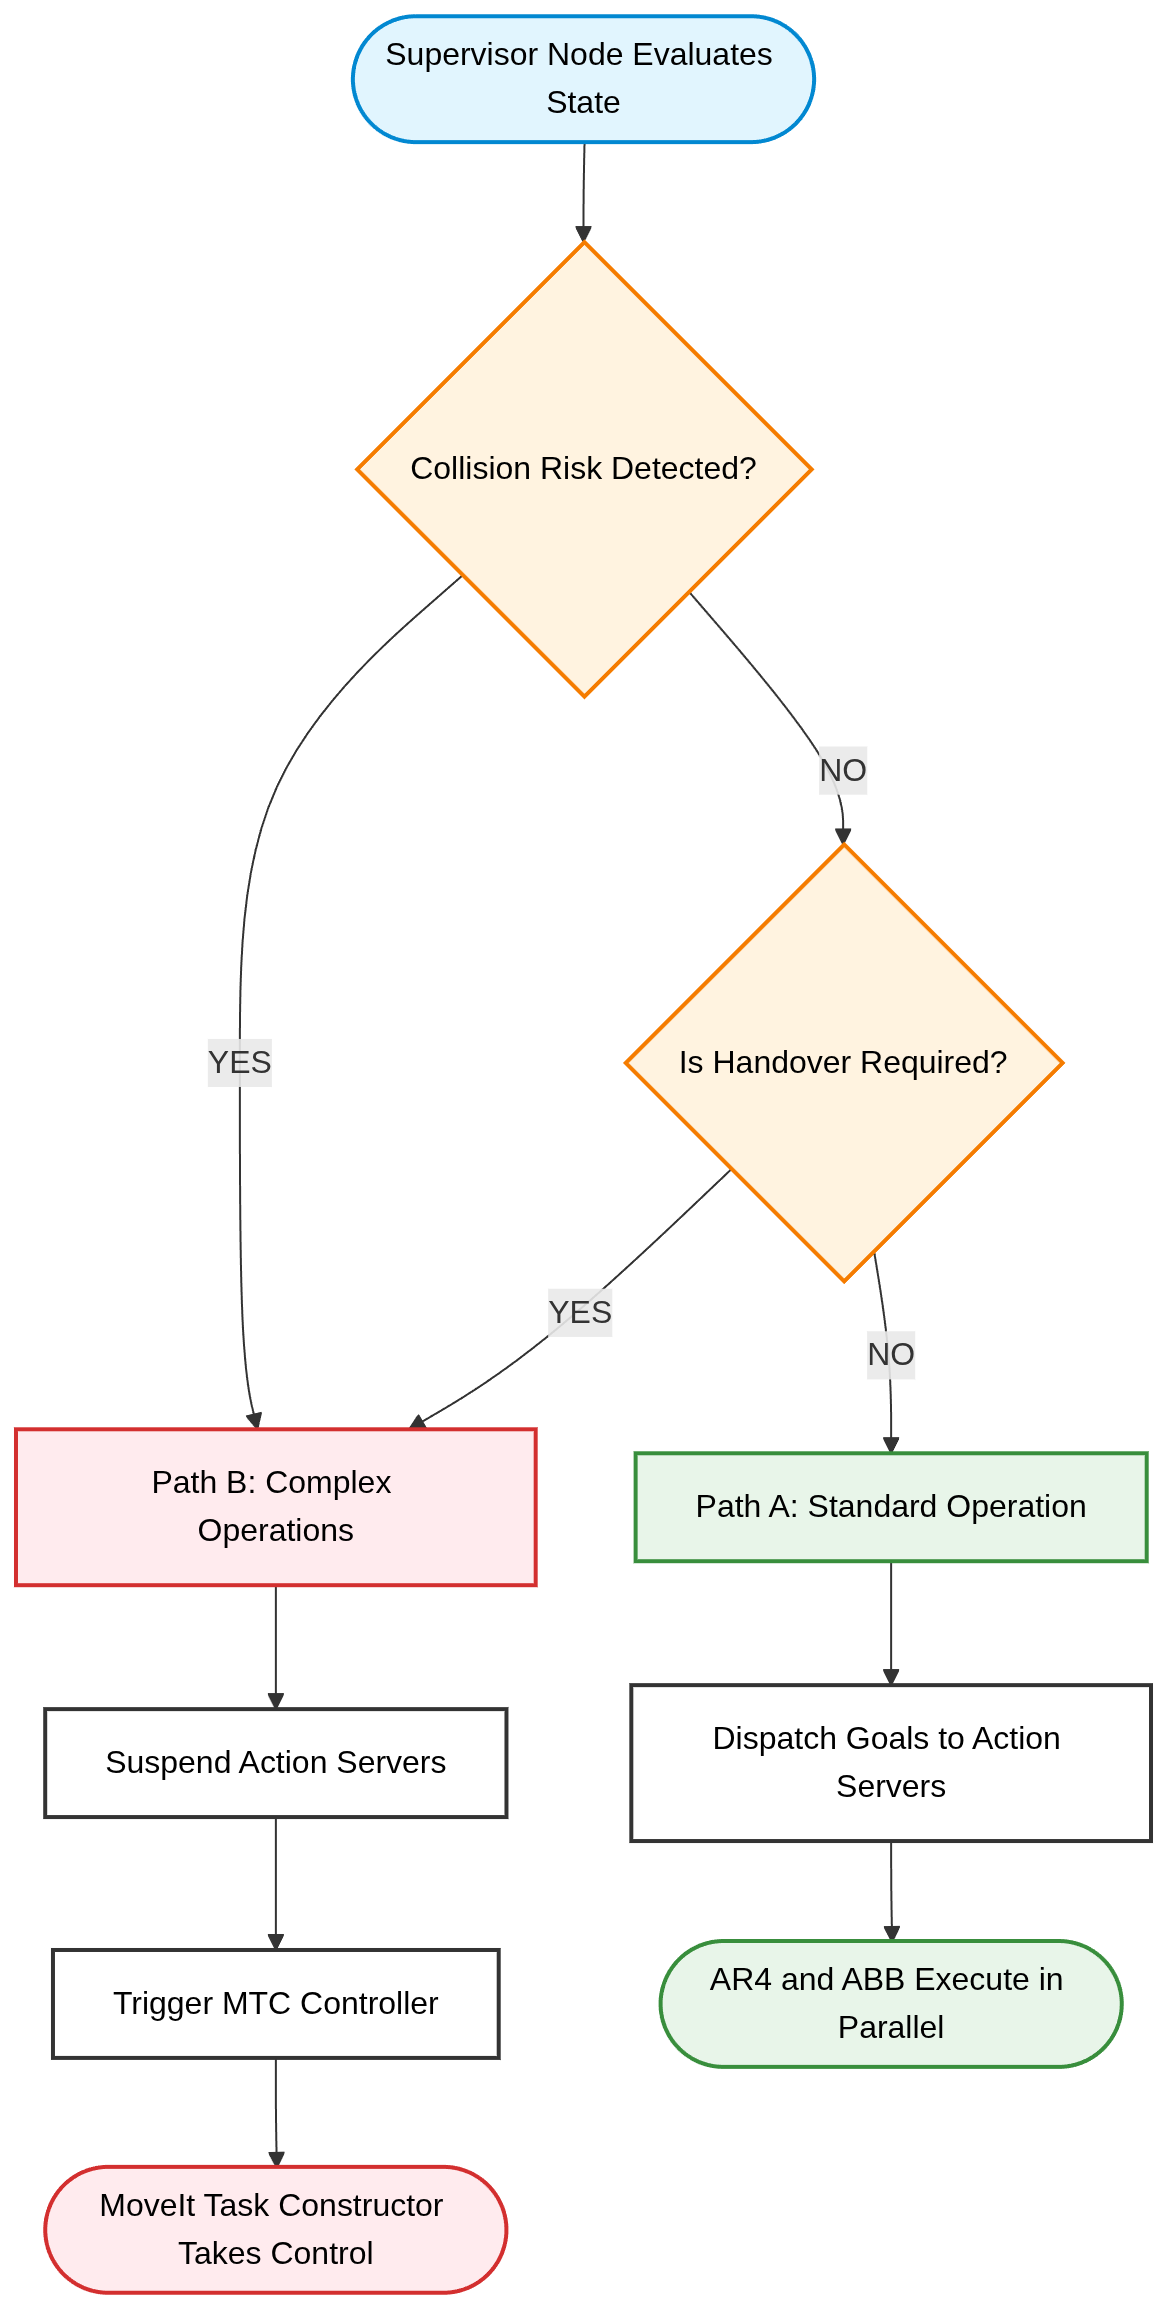
\includegraphics[width=0.52\textwidth]{figures/chapter3/ch3_mtc/Hybrid_Mode_Switching_Logic.png}
    \caption{Decision tree and runtime path branching for the Hybrid Operational Architecture.}
    \label{fig:mode_switching_logic}
\end{figure}

This switch occurs in two primary scenarios: orchestrating the collaborative handover and executing dynamic conflict resolution. By confining MTC to complex operations, the system avoids the computational overhead of generating massive task graphs for simple, repetitive pick-and-place maneuvers, reserving maximum CPU resources for when interdependent planning is strictly necessary.
\FloatBarrier

\subsection{Multi-Stage Planning: The Handover Sequence}
The collaborative handover is the most complex maneuver in the robotic cell, requiring precise synchronization. The \texttt{create\_collaborative\_handover\_task} function constructs a directed acyclic graph of potential solutions, breaking the sequence into discrete, verifiable stages. This linear sequence of operations is modeled as a functional pipeline in Figure~\ref{fig:mtc_handover_pipeline}.

\begin{figure}[htbp]
    \centering
    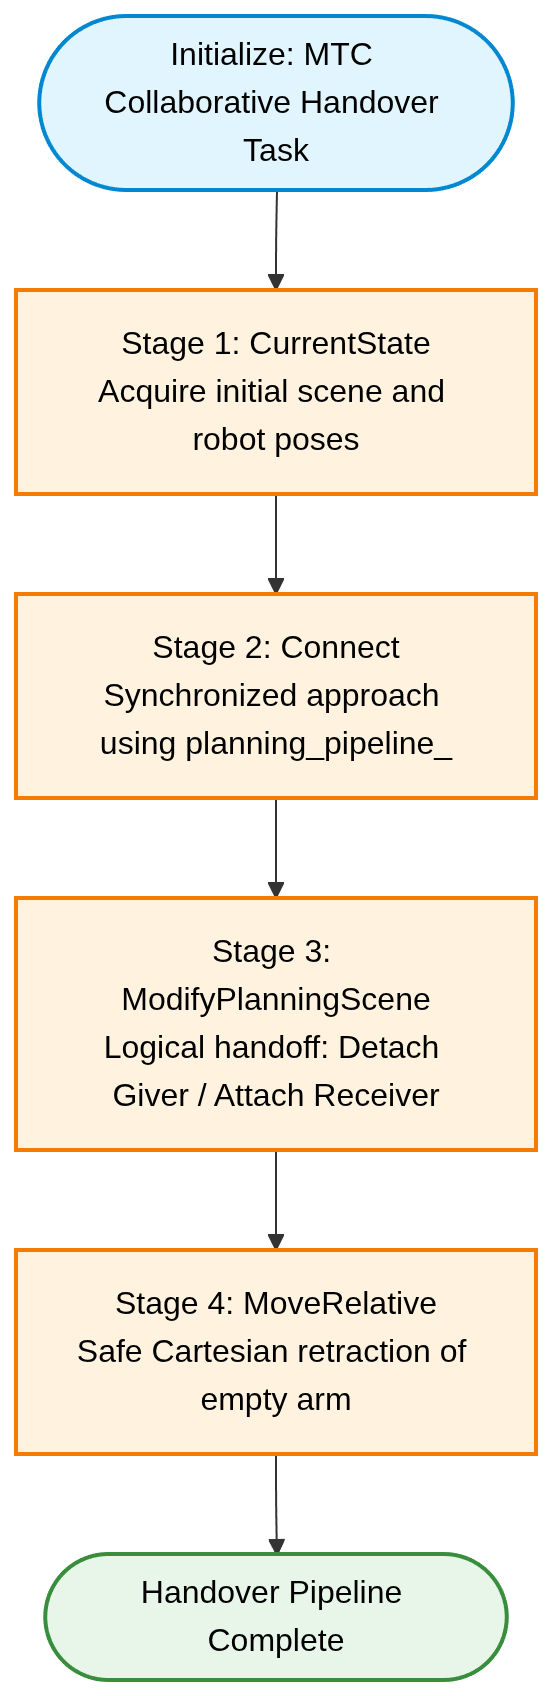
\includegraphics[width=0.28\textwidth]{figures/chapter3/ch3_mtc/MTC_Handover_Task_Graph.png}
    \caption{MoveIt Task Constructor stage pipeline for the collaborative handover sequence.}
    \label{fig:mtc_handover_pipeline}
\end{figure}

\FloatBarrier

The internal operational stages run sequentially as follows:
\begin{enumerate}
    \item \textbf{Current State Acquisition:} The task begins with a \texttt{stages::CurrentState} generator, creating a snapshot of the active planning scene, including the exact positions of both arms and the attached brick.
    \item \textbf{Synchronized Approach:} Utilizing the \texttt{planning\_pipeline\_}, the system plans simultaneous approach vectors for both arms toward the handover coordinate. Small Cartesian offsets are applied (e.g., AR4 approaches from above, ABB from below) to ensure ideal gripper presentation.
    \item \textbf{Logical Handoff (\texttt{ModifyPlanningScene}):} Instead of relying on physical sensor feedback, MTC handles the transfer purely logically. A \texttt{ModifyPlanningScene} stage is injected to detach the "brick" collision object from the \texttt{ar4\_gripper} and instantly attach it to the \texttt{abb\_gripper}. This ensures that subsequent path calculations correctly account for the brick's new volume on the receiving arm.
    \item \textbf{Safe Retraction:} Finally, a \texttt{stages::MoveRelative} stage plans a safe linear retreat for the AR4 arm away from the handover zone, ensuring it clears the newly transferred object before returning to its home position.
\end{enumerate}

\subsection{Dynamic Conflict Resolution}
Beyond scheduled handovers, MTC serves as the system's primary algorithmic fail-safe. If the Zone Detection Manager detects an imminent collision during standard parallel operations, the Supervisor halts all active trajectories and triggers the \texttt{ResolveCollision} service. The MTC node dynamically constructs a \texttt{create\_safe\_resolution\_task}. The genius of this approach lies in treating the active manipulators as dynamic obstacles:
\begin{itemize}
    \item \textbf{Phase 1:} The planner treats the ABB arm's frozen position as a static collision object and attempts to find a safe escape trajectory for the AR4.
    \item \textbf{Phase 2:} Once the AR4's new theoretical position is established, it treats the AR4 as the static obstacle and routes the ABB arm to safety.
\end{itemize}

To prevent the system from freezing due to inescapable algorithmic deadlocks, the MTC controller instantiates a localized \texttt{PipelinePlanner} with strict, hardcoded timeout constraints (e.g., 2.0 seconds). If a safe 12-DOF resolution path cannot be calculated within this window, the system defaults to a complete emergency shutdown, prioritizing hardware preservation over continued operation.